\documentclass[12pt]{spieman}  % 12pt font required by SPIE;
%\documentclass[a4paper,12pt]{spieman}  % use this instead for A4 paper
\usepackage{amsmath,amsfonts,amssymb}
\usepackage{graphicx}
\usepackage{setspace}
\usepackage{tocloft}
\usepackage[colorlinks=true, allcolors=blue]{hyperref}
\usepackage[table]{xcolor}
\usepackage{xspace}

\newcommand{\sun}{$_{\odot}$\xspace}

\DeclareRobustCommand{\ion}[2]{%
\relax\ifmmode
\ifx\testbx\f@series
{\mathbf{#1\,\mathsc{#2}}}\else
{\mathrm{#1\,\mathsc{#2}}}\fi
\else\textup{#1\,{\mdseries\textsc{#2}}}%
\fi}

\def\degr{\hbox{$^\circ$}}
\def\arcmin{\hbox{$^\prime$}}
\def\arcsec{\hbox{$^{\prime\prime}$}}
\def\utw{\smash{\rlap{\lower5pt\hbox{$\sim$}}}}
\def\udtw{\smash{\rlap{\lower6pt\hbox{$\approx$}}}}
\def\fd{\hbox{$.\!\!^{\rm d}$}}
\def\fh{\hbox{$.\!\!^{\rm h}$}}
\def\fm{\hbox{$.\!\!^{\rm m}$}}
\def\fs{\hbox{$.\!\!^{\rm s}$}}
\def\fdg{\hbox{$.\!\!^\circ$}}
\def\farcm{\hbox{$.\mkern-4mu^\prime$}}
\def\farcs{\hbox{$.\!\!^{\prime\prime}$}}


\def\aj{AJ}%

          % Astronomical Journal

\def\araa{ARA\&A}%

          % Annual Review of Astron and Astrophys

\def\apj{ApJ}%

          % Astrophysical Journal

\def\apjl{ApJ}%

          % Astrophysical Journal, Letters

\def\apjs{ApJS}%

          % Astrophysical Journal, Supplement

\def\ao{Appl.~Opt.}%

          % Applied Optics

\def\apss{Ap\&SS}%

          % Astrophysics and Space Science

\def\aap{A\&A}%

          % Astronomy and Astrophysics

\def\aapr{A\&A~Rev.}%

          % Astronomy and Astrophysics Reviews

\def\aaps{A\&AS}%

          % Astronomy and Astrophysics, Supplement

\def\azh{AZh}%

          % Astronomicheskii Zhurnal

\def\baas{BAAS}%

          % Bulletin of the AAS

\def\jrasc{JRASC}%

          % Journal of the RAS of Canada

\def\memras{MmRAS}%

          % Memoirs of the RAS

\def\mnras{MNRAS}%

          % Monthly Notices of the RAS

\def\pra{Phys.~Rev.~A}%

          % Physical Review A: General Physics

\def\prb{Phys.~Rev.~B}%

          % Physical Review B: Solid State

\def\prc{Phys.~Rev.~C}%

          % Physical Review C

\def\prd{Phys.~Rev.~D}%

          % Physical Review D

\def\pre{Phys.~Rev.~E}%

          % Physical Review E

\def\prl{Phys.~Rev.~Lett.}%

          % Physical Review Letters

\def\pasp{PASP}%

          % Publications of the ASP

\def\pasj{PASJ}%

          % Publications of the ASJ

\def\qjras{QJRAS}%

          % Quarterly Journal of the RAS

\def\skytel{S\&T}%

          % Sky and Telescope

\def\solphys{Sol.~Phys.}%

          % Solar Physics

\def\sovast{Soviet~Ast.}%

          % Soviet Astronomy

\def\ssr{Space~Sci.~Rev.}%

          % Space Science Reviews

\def\zap{ZAp}%

          % Zeitschrift fuer Astrophysik

\def\nat{Nature}%

          % Nature

\def\iaucirc{IAU~Circ.}%

          % IAU Cirulars

\def\aplett{Astrophys.~Lett.}%

          % Astrophysics Letters

\def\apspr{Astrophys.~Space~Phys.~Res.}%

          % Astrophysics Space Physics Research

\def\bain{Bull.~Astron.~Inst.~Netherlands}%

          % Bulletin Astronomical Institute of the Netherlands

\def\fcp{Fund.~Cosmic~Phys.}%

          % Fundamental Cosmic Physics

\def\gca{Geochim.~Cosmochim.~Acta}%

          % Geochimica Cosmochimica Acta

\def\grl{Geophys.~Res.~Lett.}%

          % Geophysics Research Letters

\def\jcp{J.~Chem.~Phys.}%

          % Journal of Chemical Physics

\def\jgr{J.~Geophys.~Res.}%

          % Journal of Geophysics Research

\def\jqsrt{J.~Quant.~Spec.~Radiat.~Transf.}%

          % Journal of Quantitiative Spectroscopy and Radiative Trasfer

\def\memsai{Mem.~Soc.~Astron.~Italiana}%

          % Mem. Societa Astronomica Italiana

\def\nphysa{Nucl.~Phys.~A}%

          % Nuclear Physics A

\def\physrep{Phys.~Rep.}%

          % Physics Reports

\def\physscr{Phys.~Scr}%

          % Physica Scripta

\def\planss{Planet.~Space~Sci.}%

          % Planetary Space Science

\def\procspie{Proc.~SPIE}%

          % Proceedings of the SPIE

\let\astap=\aap

\let\apjlett=\apjl

\let\apjsupp=\apjs

\let\applopt=\ao

%

\uchyph=0


\usepackage{lineno}
\linenumbers

\title{Arcus X-ray telescope performance predictions and alignment requirements}


\author[a]{Hans Moritz G\"unther$^*$}
\author[b]{Peter Cheimets}
\author[c]{Casey T. DeRoo}
\author[a,d]{Ralf K. Heilmann}


\affil[a]{MIT Kavli Institute for Astrophysics and Space Research, Cambridge, MA 02139, USA}
\affil[b]{Center for Astrophysics, Harvard-Smithsonian Astrophysical Observatory, Cambridge, MA 02138, USA}
\affil[c]{Dept. of Physics \& Astronomy, University of Iowa, Iowa City, IA 52242, USA}
\affil[d]{Space Nanotechnology Laboratory, MIT Kavli Institute for Astrophysics and Space Research, Cambridge, MA 02139, USA}


\renewcommand{\cftdotsep}{\cftnodots}
\cftpagenumbersoff{figure}
\cftpagenumbersoff{table}
\begin{document}
\maketitle

\begin{abstract}
Arcus is a concept for a Probe-class X-ray mission to deliver high-resolution FUV and X-ray spectroscopy with two separate instruments. The X-ray spectrograph (XRS) is the focus of this paper. It consists of four spectral channels arranged in a double-tilted Rowland torus geometry.  It combines cost-effective silicon pore optics (SPO) with high-throughput critical-angle transmission (CAT) gratings to achieve $R> 3000$ in a bandpass from 12-50 \AA. We present ray-tracing studies to derive performance characteristics such as the spectral resolving power and effective area, and look at the best positioning of the four channels to improve the resiliency towards misalignments and reduce the overall impact of chip gaps. We study the effect of misalignments on the performance, and present alignment requirements in six degrees of freedom for all optical elements in the XRS. We
conclude that most tolerances can be achieved with mechanical means alone.
\end{abstract}

% Include a list of up to six keywords after the abstract
\keywords{Arcus, ray-tracing, tolerances, alignment, X-ray}

% Include email contact information for corresponding author
{\noindent \footnotesize\textbf{*}Hans Moritz G\"unther,  \linkable{hgunther@mit.edu} }

% FOR SUBMISSION
\begin{spacing}{2}   % use double spacing for rest of manuscript

% For my own while writing. It's just easier to read this way
% \begin{spacing}{1}

\section{Introduction}
\label{sect:intro}  % \label{} allows reference to this section
High-resolution X-ray and UV spectroscopy open a window into the physics of the universe that often cannot be observed with any other technique. X-rays and UV can probe the hottest and most ionized gas that remains invisible in longer wavelengths because the high ionization levels do not produce observable transitions in the radio, infrared or optical. Thus, observations in the UV and X-rays probe the most energetic processes in a number of systems. A few examples are: stellar space weather \cite{2022AN....34320019B}, the accretion onto young stars, where the UV and X-rays come from the energetic infall of material from the disk onto the stellar surface; the innermost regions of the accretion disks around black holes; and the absorption of background (X-ray) light from distant, bright continuum sources by the warm-hot inter-galactic medium to find the missing baryons\cite{10.1117/12.2231193,10.1117/12.2529499}. High-resolution UV and X-ray spectroscopy that resolves the profiles of individual emission or absorption lines is particularly valuable, because it allows us to address a host of physical questions that cannot be answered by simply measuring the broad-band X-ray flux.
To follow-up with one specific example: in the case of accretion onto young stars, resolving the kinematic line profile of emission in different ions can tell us which part of the emission is formed in the infalling, red-shifted accretion column, which part is related to the stellar corona seen at the rest wavelength of the star (possibly with small velocities from up and downflows in the corona), and which part is formed in (or possibly absorbed by) the blue-shifted outflow \cite{10.1117/12.2529499}.

The Arcus mission is a concept that will address those challenges with two instruments for X-ray and UV high-resolution spectroscopy. The mission evolved through several stages. It was originally
proposed as an instrument mounted on the International Space Station\cite{10.1117/12.2062671} and then redesigned as a satellite\cite{10.1117/12.2231778,10.1117/12.2272818}. Arcus' X-ray spectrograph (XRS) will perform
high-resolution spectroscopy in the soft X-ray range (about 12-50~\AA{}) with a resolving power $R>3000$ and an effective area $A_\textrm{eff}>
300\;\mathrm{cm}^2$ for most of the bandpass with a peak close to $A_\textrm{eff} > 600\;\mathrm{cm}^2$ around 18~\AA{}. The resolving power is a factor of
$3-5$ larger than what existing instruments on Chandra or XMM-Newton can
deliver and the effective area is also significantly higher; the exact number
depends on the bandpass, e.g.\ in the crucial region around the O~{\sc vii}
He-like triplet, which is density and temperature sensitive, Arcus will reach
about two orders of magnitude more effective area than Chandra/HETG currently
has. The UV spectrograph (UVS) is described by ref.~\citenum{10.1117/12.2677948} and the UV science case is discussed by ref.~\citenum{10.1117/12.2677332}. In this work, we concentrate on the XRT.

Beginning in the very early phases of the mission design we performed
ray-tracing to verify the performance characteristics of Arcus and to
improve the design\cite{10.1117/12.2232157}; in particular in \citenum{10.1117/12.2312678,10.1117/12.2677455} we utilized ray-tracing to determine the allowable misalignments of the mechanical elements that make up Arcus. Ray-tracing is particularly well suited for the problem, because it allows an arbitrary misalignment to be introduced for any element in the optical path and it can quickly iterate over different input parameters. Since the work in \citenum{10.1117/12.2312678}, the Arcus concept has evolved yet again.


\section{Layout of the X-ray Spectrograph on Arcus}
The XRS on Arcus follows the layout of a double-tilted Rowland Spectrograph (DTRS). This concept is described in detail in Ref.~\citenum{DTRS} and summarized in this section. The XRS has four channels, each with their own separate X-ray mirror and grating petal. However, the photons from all channels are imaged onto the same set of detectors. Figure~\ref{fig:arcus} shows a rendering of the optical elements of the XRS and some photon pathways through it.

\begin{figure}
    \centering
    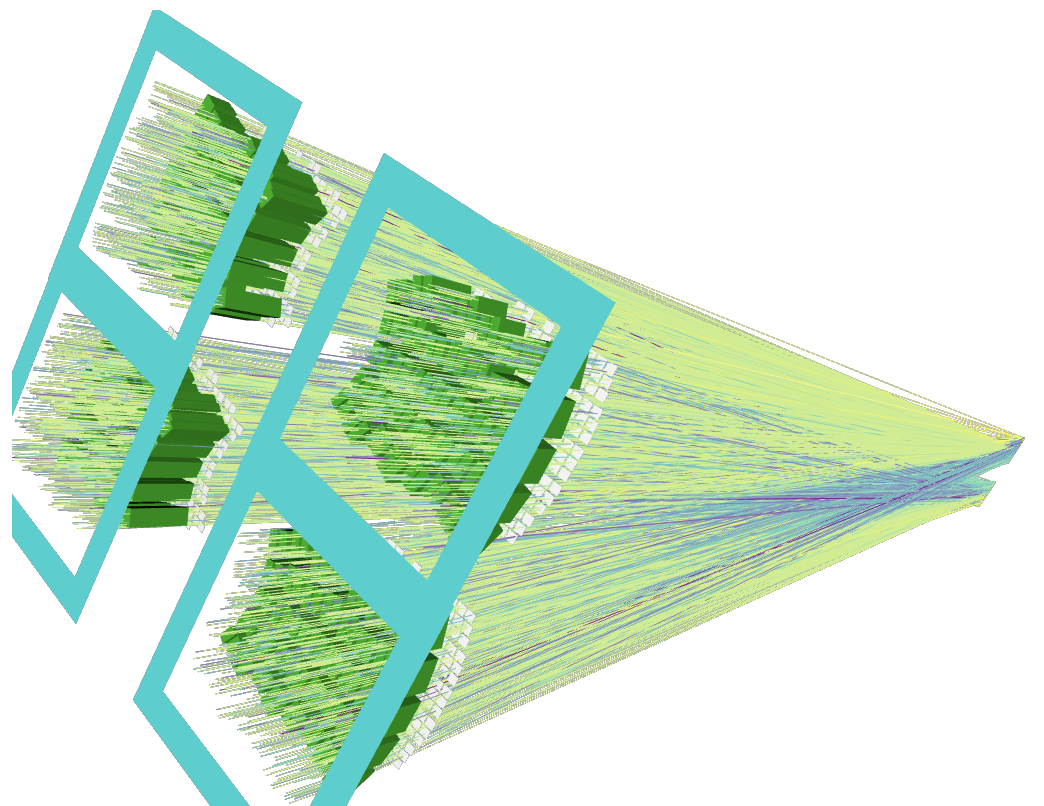
\includegraphics[height=8cm]{Arcus.png}
    \caption {\label{fig:arcus}
    Arcus to scale. On the left are the four channels with SPOs (green) and CAT gratings (white). The CCDs are in the background, where the lines converge. Lines show ray-traces. Different colors indicate different diffraction orders. Only rays that reach the detector are shown.
}
\end{figure}

\subsection{Silicon Pore Optics (SPOs)}
The SPOs are a technology developed and matured for Athena. They provide a large effective area at a relatively low weight and cost\cite{10.1117/12.2188988,10.1117/12.2599339,10.1117/12.2677388}. In Arcus, the SPO petals use ``sub-aperturing'', which means that the SPO do not cover a full circle, but only a narrow wedge. That provides Arcus with an asymmetric point-spread function (PSF) that is only about 1.5\ arcsec wide in the dispersion direction. It also means that the individual petals where the SPOs are mounted are not circular, but roughly rectangular, and four separate panels (one per optical channel) can fit into the front assembly of the telescope; see Figure~\ref{fig:arcus} for a rendering.

\subsection{Critial-Angle Transmission (CAT) gratings}
Critical-angle transmission (CAT) gratings are manufactured at the Space Nanotechnology Labo\-ra\-tory.
Progress on the development, manufacturing and x-ray performance of CAT gratings is given in a series of papers stretching back many years\cite{OE2008,AO2011,EIPBN2016,AO2019,2022ApJ...934..171H}.
CAT gratings have a very high aspect ratio, where the grating bars are about 50 times higher than they are wide. Arcus will feature CAT grating with a period of 200~nm in the dispersion direction, 140~nm gaps between the bars and a depth of 5.6~$\mu$m. The gratings are manufactured with sizes up to $32\times32$ mm$^2$. Individual grating bars are held in place by a perpendicular support structure of wider Si bars (L1 support) and a hexagonal frame (L2 support) that the gratings bars and L1 supports rest on. The L2 mesh blocks $\sim 19$\% of the area, and the recently fabricated L1 meshes block between 10 and 18\% -- see Fig.~\ref{fig:cell} for an image and a schematic.

\begin{figure} [ht]
    \begin{center}
    \begin{tabular}{c} %% tabular useful for creating an array of images
    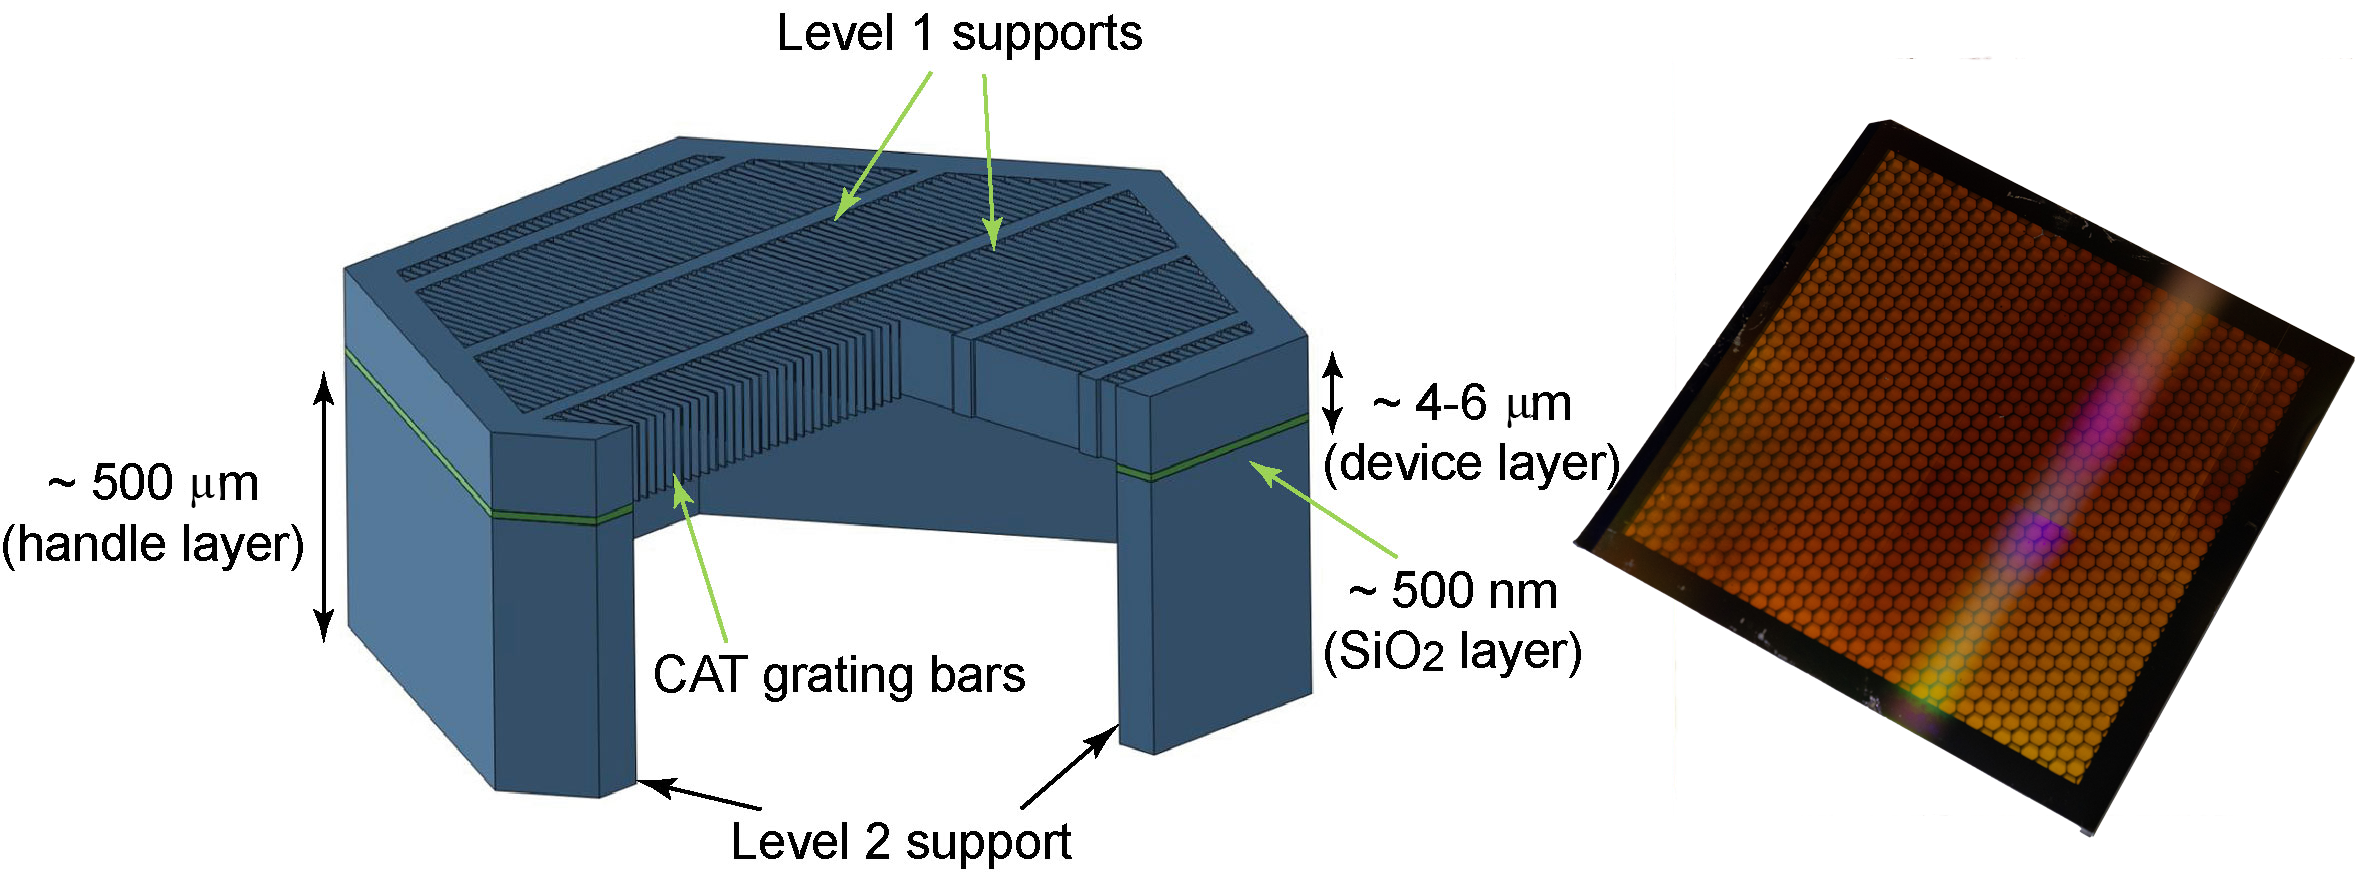
\includegraphics[height=5cm]{unitcell+pic.png}
    \end{tabular}
    \end{center}
    \caption {\label{fig:cell}
    Left: Schematic depiction of the structural hierarchy of the CAT grating membrane (see text). Right: Photograph of a back-illuminated $32\times32$ mm$^2$ prototype CAT grating membrane, showing the hexagonal L2 mesh and optical diffraction from the L1 mesh.
    }
\end{figure}

CAT gratings are mounted blazed, which means that the grating bars are not perpendicular to incoming rays, but tilted by 1.8~degrees. Together with the high aspect ratio, this leads to absolute diffraction efficiency $> 30$\%  at 2.38~nm wavelength (sum over blazed orders), including absorption by L1 and L2 supports\cite{doi:10.1117/12.2314180}. In this setup, the photons are mostly diffracted into one direction, the so-called ``blaze peak'' at twice the blaze angle.

Six CAT gratings are bonded into a window for each SPO. Those windows are then arranged into a grating petal for each channel.

\subsection{Double-tilted Rowland Torus layout}
Each channel follows a Rowland torus layout\cite{Beuermann:78} where the gratings are mounted on the surface of the torus and the detectors on the opposite side. Detectors follow the curved Rowland circle, which optimizes the width in the dispersion direction to increase the spectral resolving power of the instrument at the cost of a slightly wider photon distribution in cross-dispersion direction. For each channel, the Rowland torus is tilted by 3.6175~deg, about twice the blaze angle\cite{10.1117/12.856482,10.1117/12.2273011,DTRS}. This number is set such that the distance between two channels matches the space required to mount the grating petals next to each other. At the same time, all channels can be imaged on the same set of detectors (Fig.~\ref{fig:geometry_camera}).
The different tilted tori are arranged in such a way, that they overlap in the Rowland circle, so that the optimal detector position for one channel is also the optimal detector position for all other channels.
Two cameras are positioned to capture the zeroth order on one side and the blaze peak on the other. There is a gap between the two cameras because so little signal is found in that region that it is not useful to capture it with CCDs.

\begin{figure} [ht]
    \begin{center}
    \begin{tabular}{c} %% tabular useful for creating an array of images
    \includegraphics[width=\textwidth]{geometry_camera}
    \end{tabular}
    \end{center}
    \caption {\label{fig:geometry_camera}
    Layout of the CCDs (orange rectangles) in the focal plane. Given the resolution of the figure, most chip gaps are not visible. Also note, that the x and the y axes are scaled differently. Two cameras with eight CCDs each are located in the focal plane. In this plot, 0 is the geometric center of all the Rowland tori involved. Note that the cameras are intentionally not symmetric to 0.
    The position of the four optical axes for the four channels is marked with a blue pentagon.  The dispersion ($x$ - green horizontal arrows) and the cross-dispersion ($y$ - blue vertical arrows) of the different spectra are parallel to each other and point in the same direction. Two channels disperse left-to-right, and two right-to-left.
    }
\end{figure}

The four channels are arranged in pairs. Two of them have the zeroth order on the left in Figure~\ref{fig:geometry_camera} and disperse to the right, two of them have the zeroth order on the right and disperse towards the left. The pair of channels dispersing in the same direction set the CAT gratings on very similar Rowland tori, which are offset from each other in cross-dispersion direction by 10~mm so that the signal is clearly separated on the CCDs. They are also offset from each other in dispersion direction by 5~mm, to ensure that the same wavelength seen in different channels falls onto different x coordinates on the CCDs and thus a wavelength that happens to be lost in a chip gap between two CCDs in one channel can be observed in the other channel.

\section{RAY-TRACING}
\label{sect:raytracing}
\subsection{Optical Design}
\label{sect:design}

Each of the four channels of the XRS has a separate zero-order position and disperses the light to a different location on the detector. This has two main advantages: there is no need to align all channels to the same zero-order position within the width of the PSF (less than 1.5 arcsec in dispersion direction), and any wavelength of light that falls in a chip gap for one channel will be observable in the others; see Figure~\ref{fig:geometry_camera}. At the same time, this layout allows us to use the same detectors for all four channels, which reduces cost and complexity. More details of the optical layout are given in our previous ray-tracing papers\cite{10.1117/12.2273011,10.1117/12.2312678,DTRS}.

\section{Ray-traces}
We study the performance and alignment requirements of Arcus with ray-tracing. We use the ray-tracing code MARXS\cite{2017AJ....154..243G,marxs2.0}, a Python code developed by us under an open source license. MARXS is available at \url{https://github.com/chandra-marx/marxs}; simulations in this article are done with version 2.0. MARXS has been used for several mission proposals and is backed by hundreds of units tests and verified against laboratory works and on-orbit Chandra observations where feasible. MARXS does not calculate material properties such as reflectivities or grating efficiencies; instead they are read in from tables that can be based on laboratory data or simulations calculated by other programs.

The SPO model in the ray-trace is simplified and does not take into account vignetting, so the effective area predictions are not valid of off-axis source; but it does consider the geometric opening area (incl.\ ribs) and angle-dependent reflectivity to predict the effective area.

For CAT gratings we use efficiencies that are predicted from numerical simulations and that match the efficiencies measured for CAT gratings in the laboratory. The numbers include the effect of cross-dispersion from L1 support structures, dispersion and blockage by the hexagonal L2 supports, and any coverage by grating frames.


The cameras are covered a contamination blocking filter of 30~nm Al deposited on 45~nm polyimide and held by a thicker mesh with 95\% transmission. The mesh is treated statistically in the ray-trace as a 5\% reduction in intensity. 40~nm Al are deposited directly on the detectors to block optical light. The transmission for Al and polyiamide is taken from Ref.~\citenum{CXRO} with XAFS for C edge from measurements of Chandra ACIS imaging filter\cite{10.1117/12.245111}.
For the quantum efficiency of the CCD, we follow the QE of the Suzaku XIS1 BI CCD assuming depletion depth 42 microns\cite{2007PASJ...59S..23K}.

%;below 0.18 keV this is from ACIS S1 BI QE provided by Herman Marshall in file s1_newqe.qdp"}



\section{Effective area and resolving power}
The main performance characteristics of Arcus are the effective area and the resolving power of the extracted spectra. We run simulations on a wavelength grid from 1.5 to 60 \AA{} in steps of 0.15~\AA{}. Each simulation is run with 100,000 rays. MARXS tracks the probability of survival for each ray; for example when a ray passes a filter that transmits 15\% of the photons at that energy, the probability of a ray passing that filter is multiplied by $0.15$. In the end, the sum of the probabilities of all photons hitting the detector divided by the total number of rays simulated for a given entrance aperture gives the effective area with much lower statistical noise than in codes where photons either pass or do not pass individual elements. The uncertainty on the Arcus performance is dominated by the uncertainty in the material properties such as SPO reflectivity or CAT grating efficiency. These systematic effects are difficult to quantify, but are probably of order 10-20\% or so in sum, while the statistical uncertainty for each run is below a few per cent.

\begin{figure}
    \centering
    \includegraphics[width=0.8\textwidth]{Aeff_JATIS}
    \caption {\label{fig:Aeff}
        Effective area for Arcus based on ray-trace simulations. The effective area of individual dispersion orders is shown. For most wavelength ranges, several dispersed orders contribute to the total effective area.
    }
\end{figure}

The effective area for Arcus is shown in Figure~\ref{fig:Aeff} and the spectral resolving power $R$ per order and averaged over all orders that contribute at a particular wavelength (weighted by the effective area of each order at that wavelength) in Figure~\ref{fig:R}. The figure distinguishes between the photons seen in dispersion and in order zero, i.e.\ in direct light, where the only energy resolution is provided by the CCD. The effective area in direct light is high for high energies, in particular including the 6.7~keV (1.85~\AA{}) iron line, which is a crucial diagnostic in many astrophysical sources. Towards longer wavelengths, around 10~\AA{}, light in order 1 and -1, makes up the bulk of the signal with $R$ of a few hundred. From about 12~\AA{} to 60~\AA{} most photons are dispersed into the blaze peak on the set of detectors opposite of the zeroth order and Arcus achieves an $R$ around 3500, almost independent of wavelength. The resolving power increases with increasing distance between the location of the zeroth other and the dispersed signal. For a given order, that means that $R$ increases with wavelength. However, for most wavelengths, multiple orders contribute to the signal. As the wavelength increases, the order on the far side of the blaze peak becomes weaker, and orders on the near side stronger, such that the average $R$ is approximately constant.


\begin{figure}
    \centering
    \includegraphics[width=0.8\textwidth]{R_JATIS}

    \caption {\label{fig:R}
    Resolving power $R$ for Arcus. Colored lines show $R$ per order, the gray area shows $R$ averaged over all diffracted orders contributing to that wavelength, where the average is calculated weighting each order by the effective area. For low orders, there are gaps in the colored lines. At low wavelength, those orders fall on the same camera as the zeroth order, e.g.\ for order -2 up to 20~\AA{}. In order -2 photons longer than 43~\AA{} are dispersed into the blaze peak and detected on the other camera.
    }
\end{figure}

\section{Alignment tolerances}
We use ray-traces to assess the effect of misalignments on the performance of Arcus. Science requirements put limits on the maximal allowable degradation of spectral resolving power and effective area, and engineering constraints determine how well e.g.\ individual SPOs can be aligned into petals, how well the petals can be aligned to the forward assembly, and how well the forward assembly can be aligned to the detector housing. In general, tighter tolerances require more work, time, and money. We thus need to understand how important each possible degree of freedom is to the total performance of the system to identify those where significant design and work needs to go into the alignment.

The simulations start from a perfectly aligned version of Arcus. Even this does not provide infinite resolving power, because the model includes pointing jitter, a limited PSF, some astigmatism inherent in the design, and finite sizes of CAT gratings and CCD detectors, which means that they deviate from the ideal Rowland geometry. A ray-trace is run with this design and spectral resolving power ($R$) and effective area ($A_\mathrm{eff}$) are calculated.

After running the baseline version, one element of Arcus is shifted in one degree of freedom, e.g.\ all CCDs are shifted by 1~mm in the dispersion direction. The ray-trace is repeated, again $R$ and $A_\mathrm{eff}$ are calculated, then all CCDs are shifted by 2~mm and so on. After testing out the parameter space in dispersion direction, the CCDs will be shifted in cross-dispersion direction. In this way, each element (for example, the CCD array), will be misaligned by various amounts in one of 6 degrees of freedom (shift along $x$, $y$, $z$, and rotation around $x$, $y$, $z$).
In the Arcus coordinate system, the $z$-axis is parallel to the optical axis, the $x$-axis is the grating dispersion direction and the $y$-axis is the cross-dispersion direction. Unless noted, rotations are not done around the origin of the coordinate system, but around the center of an element (e.g.\ the center of a SPO petal).

In the first stage, only one degree of freedom is changed at a time, because it is not computationally feasible to explore the entire parameter space. From those results, we identify where the alignment is easily (e.g.\ just from simple machining tolerances) much better than the requirements. In a second step, we can then run ray-traces where all degrees of freedom are varied according to the misalignment budget and thus check if the assumptions going into combining the misalignments in different degrees of freedom hold or if non-linear interactions degrade $R$ and $A_\mathrm{eff}$ more than expected. Should this be the case, we revise the misalignment budget appropriately.

To keep the computational load reasonable, we simulate only one channel of Arcus. Since spectra from each channel will be extracted separately and there is symmetry between the channels, most results apply equally to all channels. We discuss in the text the few instances where the channel symmetry does not apply.
Each simulation consists of 200000 photons and the same source photons are used for each series of ray-traces, e.g.\ all global CCD misalignments use the same photons.

\begin{figure} [ht]
    \begin{center}
    \begin{tabular}{c} %% tabular useful for creating an array of images
    \includegraphics[width=0.7\textwidth]{CAT_global_JATIS}
    \end{tabular}
    \end{center}
    \caption {\label{fig:CAT_global}
    Effect of mislignment of the CAT grating petal for rotation around the center of the petal. (a-c): Resolving power for rotation around $x$, $y$, and $z$, respectively, (d-f): effective area for rotation around $x$, $y$, and $z$, respectively.
    }
\end{figure}
\begin{figure} [ht]
    \begin{center}
    \begin{tabular}{c} %% tabular useful for creating an array of images
    \includegraphics[width=0.7\textwidth]{CAT_individual_JATIS}
    \end{tabular}
    \end{center}
    \caption {\label{fig:CAT_individual}
    Effect of mislignment of individual CAT gratings. The mislignment for each grating is drawn from a normal distribution, the $\sigma$ of that distribution varied from 0 to 3~degrees. (a-c): Resolving power for rotation around $x$, $y$, and $z$, respectively, (d-f): effective area for rotation around $x$, $y$, and $z$, respectively. Note that the $A_\mathrm{eff}$ reported is only for a single channel.
    }
\end{figure}
\begin{figure} [ht]
    \begin{center}
    \begin{tabular}{c} %% tabular useful for creating an array of images
    \includegraphics[width=0.7\textwidth]{detector_global_JATIS}
    \end{tabular}
    \end{center}
    \caption {\label{fig:detector_global}
    Effect of mislignment the cameras with respect to the front assembly. (a-c): Resolving power for translation parallel to $x$, $y$, and $z$, respectively, (d-f): effective area for translation parallel to $x$, $y$, and $z$, respectively.
    }
\end{figure}

Figures~\ref{fig:CAT_global}, \ref{fig:CAT_individual}, and \ref{fig:detector_global} show some examples of the results. In the figures, $A_\mathrm{eff}$ is given summed over all dispersed orders that fall on a CCD (bottom row) and $R$ is the average resolving power, where the resolving power from individual orders is averaged weighted by the number of photons in that particular order (top row). Thus, it is possible, that $R$ in the plot increases with increasing misalignment if $A_\mathrm{eff}$ drops at the same time. This happens when an order with lower-than-average $R$ drops off the CCD (thus reducing the summed $A_\mathrm{eff}$ and increasing the average $R$). There is no scientific benefit from the apparently increased $R$ here - if one required a higher resolving power, the lower orders can be ignored in scientific analysis even if they fall on the CCD.


Figure~\ref{fig:CAT_global} shows the effect of a change in the CAT grating petal position, while the SPO petal and the cameras are fixed. Rotations around either $x$ or $y$ mean that the CAT gratings on one side move up, while the other side moves down, changing the path length of the diffracted photons. Those photons coming from the high CAT gratings travel further along the dispersion direction than those from the low gratings, thus causing the dispersed spot to smear out, which reduces $R$. These rotations need to be kept at the level of a few arcminutes. Rotation around $z$ changes the direction of the dispersed light and, for large angles, the dispersed orders miss the CCD.

Figure~\ref{fig:CAT_individual} examines the rotations of individual gratings. For each grating in the CAT petal, a different misalignment is drawn from a normal distribution. Rotations around $x$ (the dispersion direction, see panels a and d in the figure) have little effect on $R$. Since the flat facets have finite size, their edges differ from the Rowland torus by a little already, and adding a little more rotation does not change much. Rotations in $y$ quickly reduce $A_\mathrm{eff}$ though, because the CCDs are placed for a certain blaze peak. Rotating the CAT gratings shifts the blaze peak and photons miss the CCDs. Rotation around $z$ causes more and more signal to miss the detector. There is no sharp cut-off, because the CAT gratings in the simulation have a distribution of rotation angles, and the larger the Gaussian $\sigma$ is, the more CAT gratings will send their dispersed photons to positions where they cannot be detected. From this figure, we can determine that the alignment tolerance for rotation around $x$ can be large, while the other two directions are of order a few arcminutes to prevent significant degradation of the Arcus performance.

Figure~\ref{fig:detector_global} shows simulations for translating the detector with respect to the forward assembly (SPOs and CAT gratings). The most important degree of freedom is a change in focus (panel c). A shift along $y$ has no impact, as long as it is small enough to keep the dispersed spectrum on the CCDs. For the particular channel simulated here, the spectrum drops off the CCDs for $y$ shifts for about -15~mm on one side and about +5~mm on the other side. A shift of 5~mm or more will drop at least one channel of the detector.

The curves for changing $R$ with shift in $x$ show some up and down when an order hits a chip gap (panel a and d). For example, two orders contribute to the signal in the curve for 37~\AA{} photons. At +2 mm one of them hits a chip gap, causing a drop in $A_\mathrm{eff}$ and also in $R$ ($R$ is averaged over all contributing orders, but only one order, which happens to have a lower $R$, is detected at this position). Note that chip gaps are inevitable. There will always be some wavelengths in a chip gap; however, the overall performance of the instrument, which is averaged over a range of wavelengths, is unaffected by this. While, in principle, a shift along $x$ does matter in principle since the focal plane is curved, we find that shifts up to a few mm have little impact, as if the CCDs move in the dispersion direction, the spectrum will be only slightly out of focus. As described above, the Arcus design takes advantage of this to mitigate the effect of chip gaps by offsetting the different channels by a few mm in dispersion direction so that no two spectra have chip gaps at the same wavelength.

We run simulations for rotations and translations for each possible mechanical misalignment in Arcus, as well as for a few other parameters such as the SPO mirror PSF, the repeatability of the CAT grating period, the surface flatness of the CAT gratings etc. Inspecting all results, and considering how easy or hard it is to improve alignments in each degree of freedom, we set the alignment tolerances listed in Table~\ref{tab:tolerances}.

\begin{table}
    \caption{Arcus alignment tolerances ($1\sigma$)\label{tab:tolerances}}
    \centering
    \begin{tabular}{l|cccccc}
        \hline\hline
    alignment & trans x & trans y & trans z & rot x & rot y & rot z \\
     & $\mathrm{mm}$ & $\mathrm{mm}$ & $\mathrm{mm}$ & $\mathrm{{}^{\prime\prime}}$ & $\mathrm{{}^{\prime\prime}}$ & $\mathrm{{}^{\prime\prime}}$ \\
     \hline
    individual SPO in petal & 0.007 & 0.033 & 0.167 & 100 & 100 & 3 \\
    CAT petal to SPO petal & 0.333 & 0.333 & 0.333 & 100 & 100 & 200 \\
    CAT windows to CAT petal & 0.333 & 0.333 & 0.067 & 100 & 60 & 100 \\
    individual CAT to window & 0.333 & 0.333 & 0.067 & 100 & 60 & 100 \\
    Camera to front assembly & 1.667 & 0.667 & 0.333 & 60 & 60 & 200 \\
    \end{tabular}
\end{table}

The alignment budget assumes that all alignment tolerances contribute independently. The next set of simulations is designed to check this assumption. Some misalignments might cancel out in practice, others might have a multiplicative effect. Full ray-tracing is the best way to check that and to predict final instrument performance. We run a set of 100 ray-traces, and draw a new set of mislaignments from Table~\ref{tab:tolerances} for each of them. Figure~\ref{fig:alignment_budget} shows the cumulative distribution of $R$ and effective area for those simulations relative to a perfectly aligned Arcus.

\begin{figure}
    \centering
    \includegraphics[width=0.75\textwidth]{alignbudget_base}
    \caption {\label{fig:alignment_budget}
    Cumulative distribution function for $R$ (panel a) and effective area (panel b) relative to a perfectly aligned Arcus for a set of simulations where all elements are simultaneously misaligned according to the misalignment budget in Table~\ref{tab:tolerances}.}
\end{figure}


Differences are visible between the different wavelengths. At 37~\AA{} two dispersed orders (order -3 and -4) contribute, but order -3 is close to the edge of a CCD and order -4 is close to a chip gap. If either one is lost, $R$ or $A_\mathrm{eff}$ at that wavelength will suffer, but at the same time a neighboring wavelength will improve because it is no longer inside a chip gap. In contrast, the signal at 25~\AA{} is dominated by order -6, comfortably in the middle of a CCD. Thus, the two plots above should not be interpreted as ``longer wavelength will suffer more''; crucial orders are close to a chip gap in different spots over the Arcus bandpass. Instead, the plots should be read as showing the range of effects that the baseline misalignment can have on $R$ and $A_\mathrm{eff}$, depending on what exactly the random numbers are that are drawn.

Apart from the effects of shifting chip gaps, Figure~\ref{fig:alignment_budget} shows that the alignment tolerances listed in Table~\ref{tab:tolerances} give us 95\% of the nominal $R$ and effective area in more than 90\% of the realizations.

We use the feedback we gain from our ray traces to revisit the error budget and look for places where we can relax it without impacting performance.
For example, we have been able to relaxe rotational alignment tolerances for CAT grating membranes and/or facets to their grating window by a factor of three relative to Table 1 with acceptable minimal impact on XRS performance.

\section{Future Work}
At this point, the main limitation of this work is our simplified mirror model. We expect it to work well for on-axis sources, but it does not reproduce the vignetting which becomes significant at about 2~arcmin. Our simplified mirror model also leads to a flat focal plane, while a Wolter-Schwarzschild optic typically has a slightly curved focal surface. Detailed ray-trace models specific to the Athena SPOs are available\cite{10.1117/12.2232230,10.1117/12.2594461,10.1117/12.2628133} and can be coupled with our code for CAT gratings and detectors.

\section{Summary}
\label{sect:summary}
Arcus is a Probe-class mission concept with two high-resolution spectrographs in the UV and in X-rays. The X-ray instrument (XRS) is designed in a double-tilted Rowland torus geometry with four channels with independent mirror and grating petals. All four channels are imaged onto the same set of detectors. We discuss the ray-racing model we set up for Arcus and describe the input data for mirrors, gratings, filters, and CCDs. We predict an effective area of $>200$~cm$^2$ from 8-50~\AA{} with a peak of 550~cm$^2$ around 15~\AA{}. The resolving power $R$ is largely flat over the bandpass with $R>3500$. Arcus will also detect higher-energy X-rays up to 10~keV in low diffraction orders (-1, 0, and +1) at the same time.

We run simulations to determine the alignment tolerances for Arcus. In many degrees of freedom, those are of order 0.5~mm for translations or 1-2~arcmin for rotations, which is easily achievable by mechanical means alone. Notably, the alignment requirements of individual SPOs in a mirror petals  and the translation of the CAT windows and petals along the optical axis are tighter and require dedicated alignment procedures.






% \disclosures
\subsection*{Disclosures}
The authors of this paper are members of the Arcus collaboration; R.~Smith is the PI of Arcus, A.~Ptak is the Co-PI, all other authors are Co-Is. Should NASA select Arcus for implementation, their institutions will receive funding which may be used to fund the author's salaries in full or in part in the future.


\subsection* {Code, Data, and Materials Availability}
We use the ray-tracing code MARXS\cite{2017AJ....154..243G,marxs2.0}, a Python code developed by us under an open source license. MARXS is available at \url{https://github.com/chandra-marx/marxs}; simulations in this article are done with version 2.0. The database of efficiencies for gratings is considered a trade secret by the Space Nanotechnology Laboratory and cannot be shared in open repositories - contact co-author Ralf Heilmann for access.


%In support of open scientific exchange, SPIE journals require Code, Data, and Materials Availability Statements in all accepted papers. This requirement went into effect on 1 May 2023. These statements should describe how to access any data that would be required to replicate or interpret the findings reported in the paper. Authors are encouraged to make the data and code related to the manuscript publicly available whenever possible, and utilize repositories that are well-known to the field (FigShare, Github, CodeOcean, etc.). If the data or code cannot be made publicly available, the authors should state the reason and explain how it can be obtained. Likewise, if data sharing is not applicable, the statement must say so. Example statements may be found in the Author Guidelines for the journal.


\subsection* {Acknowledgments}
Support
for this work was provided in part through NASA grant NNX17AG43G and
Smithsonian Astrophysical Observatory (SAO) contract SV3-73016 to MIT
for support of the {\em Chandra} X-Ray Center (CXC), which is operated
by SAO for and on behalf of NASA under contract NAS8-03060.  The
simulations make use of Astropy, a community-developed core Python
package for Astronomy\cite{astropy:2022}, numpy\cite{numpy}, and IPython\cite{IPython}.


%%%%% References %%%%%

\bibliography{report_with_doi}   % bibliography data in report.bib
\bibliographystyle{spiejour}   % makes bibtex use spiejour.bst

%%%%% Biographies of authors %%%%%
\subsection*{Biographies}
\vspace{2ex}\noindent\textbf{Hans Moritz G\"unther} is a research scientist at MIT. He received his undergraduate degree (in 2005) and his PhD (in 2009) in physics from the University of Hamburg, Germany. After that, he worked at the Harvard-Smithsonian Center for Astrophysics and came to MIT in 2015. He is currently the lead developer of MARX, the ray-tracing software used for the Chandra X-ray observatory. His science interests are in star formation using data from the radio to X-rays.

\vspace{1ex}
\vspace{2ex}\noindent\textbf{Peter Cheimets}
Peter Cheimets received a BS in Mechanical Engineering in 1978 from MIT, and a MS in Mechanical Engineering with concentrations in dynamics and control systems from Stanford in 1981. He received a management of engineering degree from Tuft in 2007. He has developed astrophysical instrumentation for the Smithsonian Astrophysical Observatory since 1983, placing instruments on TRACE, Hinode, SDO, and IRIS, and is leading the effort to develop an instrument for MUSE.

\vspace{1ex}
\vspace{2ex}\noindent\textbf{Casey DeRoo}
Casey DeRoo received his BA degree in physics and classical studies in 2011 and his PhD in physics from University of Iowa in 2016. He served as an Astrophysicist at the Smithsonian Astrophysical Observatory. He joined the faculty of the University of Iowa as an assistant professor in 2018, and was named a NASA Astrophysics Nancy Grace Roman Technology Fellow in 2020. His research interests include X-ray optics technologies, nanofabrication, and metrology.


\vspace{1ex}
\vspace{2ex}\noindent\textbf{Ralf K.~Heilmann} is a principal research scientist at the MIT Kavli Institute for Astrophysics and Space Research, and the associate director of the Space Nanotechnology Laboratory (SNL).  He received his Diplom in physics from the FAU Erlangen/N\"urnberg (1991), and his MS (1993) and PhD (1996) in physics from Carnegie Mellon University.  After a postdoc at Harvard he joined the SNL and has since focused on advanced lithography and the development of x-ray optics for astronomy.

%\vspace{1ex}
%\vspace{2ex}\noindent\textbf{Eric D. %Miller}
%Please send me your biography (approx 75 words).

%\vspace{1ex}
%\vspace{2ex}\noindent\textbf{Andrew Ptak}
%Please send me your biography (approx 75 words).

%\vspace{1ex}
%\vspace{2ex}\noindent\textbf{Randall K. Smith}
%Please send me your biography (approx 75 words).


%\noindent Biographies and photographs of the other authors are not available.



%\subsubsection{Reference linking and DOIs}
%A Digital Object Identifier (DOI) is a unique alphanumeric string assigned to a digital object, such as a journal article or a book chapter, that provides a persistent link to its location on the internet. The use of DOIs allows readers to easily access cited articles. Authors should include the DOI at the end of each reference in brackets if a DOI is available. See examples at the end of this manuscript. A free DOI lookup service is available from CrossRef at \\\linkable{http://www.crossref.org/freeTextQuery/}. The inclusion of DOIs will facilitate reference linking and is highly recommended.

%In the present LaTeX template, the author needs to add the DOI reference by including it in a ``note'' in the bibliography file, as shown in the file {\verb+report.bib+}, for example, \\ {\verb+note = "[doi:10.1117/12.154577]"+}. The DOI may be used by the reader to locate that document with the link: {\verb+http://dx.doi.org10.1117/12.154577+}.


\listoffigures
\listoftables

\end{spacing}
\end{document}